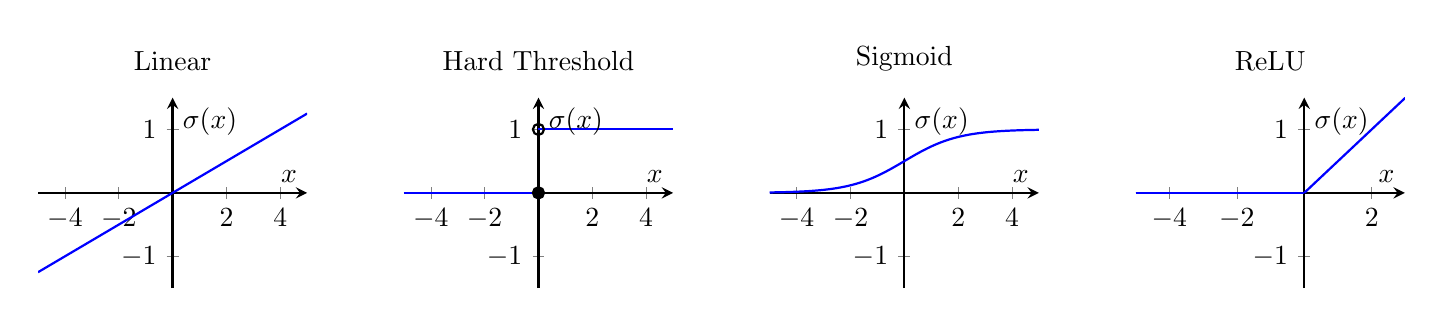
\begin{tikzpicture}[
    every axis/.style={
        width=5cm,
        height=4cm,
        % grid=major,
        axis lines=middle,
        xlabel={$x$},
        ylabel={$\sigma(x)$},
        samples=100,
        domain=-5:5,
        ymin=-1.5, ymax=1.5,
        % xtick={-4,-2,0,2,4},
        ytick={-1,0,1},
        thick
    }
]

% Arrange the four plots in a 1x2 grid
\matrix[column sep=1.2cm, row sep=1.2cm]{

% ---------- Linear ----------
\begin{axis}[title={Linear}]
    \addplot[blue] {x/4}; % scaled down for visibility
\end{axis}
&
% ---------- Hard Threshold ----------
\begin{axis}[title={Hard Threshold}]
    \addplot[blue, domain=-5:0] {0};
    \addplot[blue, domain=0:5] {1};
    \addplot[only marks, mark=*] coordinates {(0,0)};
    \addplot[only marks, mark=o, fill=white] coordinates {(0,1)};
\end{axis}
&
% ---------- Sigmoid ----------
\begin{axis}[title={Sigmoid}]
    \addplot[blue] {1/(1 + exp(-x))};
\end{axis}
&
% ---------- ReLU ----------
\begin{axis}[title={ReLU}]
    \addplot[blue, domain=-5:0] {0};
    \addplot[blue, domain=0:5] {x/2};
\end{axis}
\\
};

\end{tikzpicture}